\newpage
\section{A Parabola from an Envelope of Tangents}

In this activity, we will see that our ``cross-connecting'' method of
drawing an envelope of tangents actually draws a parabola.

\begin{prob}
Consider the grid below:
\[
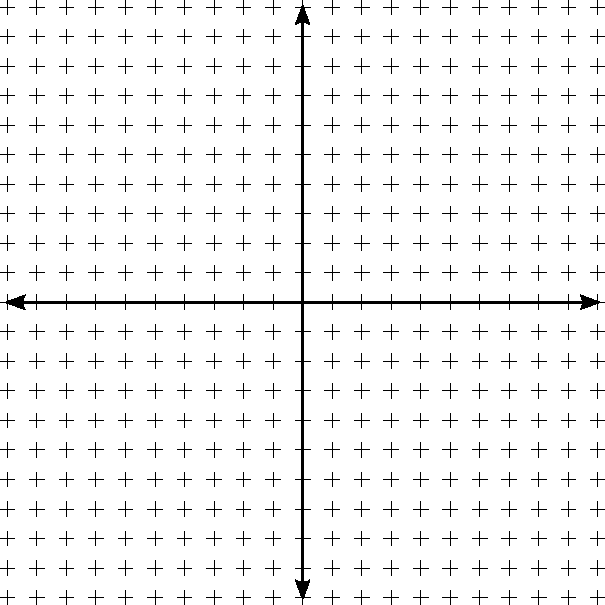
\includegraphics{../graphics/axis.pdf}
\]
Setting each square to be $1/2$ a unit, carefully plot the lines $f(x)
= 4x-4$ and $g(x) = -4x-4$.
\end{prob}

\begin{prob}
Using the two lines above, consider the segments that go from $(2,4)$
to $(0,-4)$ and from $(-2,4)$ to $(0,-4)$. Carefully draw a $7$-line
envelope of tangents using these segments.
\end{prob}

\begin{prob}
Here are two points:
\[
\vec{a} = (t,f(t)) \qquad \text{and}\qquad \vec{b}=(t-2, g(t-2))
\]
\begin{enumerate}
\item  What relevance do these points have with the plot above? 
\item Give three values of $t$ that directly relate these points to what you have
already drawn.
\item Find the equation of the line connecting $\vec{a}$ and $\vec{b}$. Call it $\l_1(x)$. 
\end{enumerate}
\end{prob}

\begin{prob}
Here are two more points:
\[
\vec{c} = (t+\ep,f(t+\ep)) \qquad \text{and}\qquad \vec{d}=(t-2+\ep, g(t-2+\ep))
\]
The Greek letter $\ep$ is our way of making a new line in our
envelope of tangents. Set $\ep = 1/2$ and see if you can answer the
questions below:
\begin{enumerate}
\item  What relevance do these points have with the plot above? 
\item Give three values of $t$ that directly relate these points to what you have
already drawn.
\item Forgetting that $\ep = 1/2$, find the equation of the line connecting $\vec{c}$ and $\vec{d}$. Call it $\l_2(x)$
\end{enumerate}
\end{prob}


\begin{prob}
Solve 
\[
\l_1(x) = \l_2(x)
\]
for $x$, and set $\ep = 0$. What do you find? What do you get when you
plot this?
\end{prob}
